\documentclass[12pt]{article}

\usepackage[utf8x]{inputenc}
\usepackage{amsmath}
\usepackage{amssymb}
\usepackage{amsfonts}
\usepackage{graphicx}
\usepackage{tikz,tkz-tab}
\usepackage{mathrsfs}
\usepackage{listings,chngcntr}
\usepackage[left=2cm,right=2cm,top=2cm,bottom=2cm]{geometry}
\usepackage{multicol}
\usepackage{float,graphicx}
\usepackage{pstricks,pst-all,pst-plot,pstricks-add,pst-3dplot}
\usepackage{cases}
\usepackage{array}
\usepackage[shortlabels]{enumitem}
\usepackage{eurosym}
\usepackage{bbm}
\usepackage[european, straightvoltages, RPvoltages]{circuitikz}
\usepackage{diagbox}

\definecolor{mygreen}{RGB}{28,172,0} % color values Red, Green, Blue
\definecolor{mylilas}{RGB}{170,55,241}

\title{CS221 - TP2}
\author{Vincent MOUCADEAU - Rémi MAZZONE | 2A}
\date{30/11/2022}


\newenvironment{restoretext}%
    {
     \begin{adjustwidth}{}{\leftmargin}%
    }{\end{adjustwidth}
     }
     
\renewcommand*{\overrightarrow}[1]{\vbox{\halign{##\cr 
  \tiny\rightarrowfill\cr\noalign{\nointerlineskip\vskip1pt} 
  $#1\mskip2mu$\cr}}}


\newcommand{\dvec}[1]{\overrightarrow{#1}} % Commande perso pour vecteurs
\newcommand{\fracvec}[3]{\dfrac{#1}{#2}\dvec{#3}}

     
\newcommand*\Vc[2][1ex]{\Vcaux#2,,\Vcaux{#1}}% arg optionnel = espacement entre coordonnées
\def\Vcaux#1,#2,#3,#4\Vcaux#5{%
    \ensuremath{\left(\vcenter{\baselineskip0pt
    \halign{\hfil\kern.25em$##$\kern.25em\hfil\crcr
        #1\cr\noalign{\vskip#5}#2\cr\noalign{\vskip#5}#3\crcr}%
    }\right)}%
} 

\newcolumntype{R}[1]{>{\raggedleft\arraybackslash }b{#1}}
\newcolumntype{L}[1]{>{\raggedright\arraybackslash }b{#1}}
\newcolumntype{C}[1]{>{\centering\arraybackslash }b{#1}}

\renewcommand{\arraystretch}{1.4}

% -------- PYTHON -------- %
\definecolor{dkgreen}{rgb}{0,0.6,0}
\definecolor{gray}{rgb}{0.5,0.5,0.5}
\definecolor{mauve}{rgb}{0.58,0,0.82}

\lstdefinestyle{languageC}{
    language=C,
    aboveskip=3mm,
    belowskip=3mm,
    basicstyle={\small\ttfamily},
    breaklines=true,%
    keywordstyle=\color{blue},%
    morekeywords=[2]{1}, keywordstyle=[2]{\color{black}},
    identifierstyle=\color{black},%
    stringstyle=\color{mylilas},
    commentstyle=\color{mygreen},%
    showstringspaces=false,%without this there will be a symbol in the places where there is a space
    numbers=left,%
    numberstyle={\tiny \color{black}},% size of the numbers
    numbersep=14pt, % this defines how far the numbers are from the text
    emph=[1]{for,end,break},emphstyle=[1]\color{red}, %some words to emphasi
    frame=single,
    frameround={t}{t}{t}{t},
    xleftmargin=.2\textwidth, xrightmargin=.2\textwidth
}

\lstdefinestyle{languageClarge}{
    language=C,
    aboveskip=3mm,
    belowskip=3mm,
    basicstyle={\small\ttfamily},
    breaklines=true,%
    keywordstyle=\color{blue},%
    morekeywords=[2]{1}, keywordstyle=[2]{\color{black}},
    identifierstyle=\color{black},%
    stringstyle=\color{mylilas},
    commentstyle=\color{mygreen},%
    showstringspaces=false,%without this there will be a symbol in the places where there is a space
    numbers=left,%
    numberstyle={\tiny \color{black}},% size of the numbers
    numbersep=14pt, % this defines how far the numbers are from the text
    emph=[1]{for,end,break},emphstyle=[1]\color{red}, %some words to emphasi
    frame=single,
    frameround={t}{t}{t}{t},
    xleftmargin=.04\textwidth, xrightmargin=.04\textwidth
}

\lstdefinestyle{pseudoCode}{
    aboveskip=3mm,
    belowskip=3mm,
    basicstyle={\small\ttfamily},
    breaklines=true,
    morekeywords={input, output, pour, si, echanger, fin, alors, faire},
    keywordstyle=\color{blue},%
    morekeywords=[2]{1}, keywordstyle=[2]{\color{red}},
    identifierstyle=\color{black},%
    stringstyle=\color{mylilas},
    commentstyle=\color{mygreen},%
    showstringspaces=false,%without this there will be a symbol in the places where there is a space
    numbers=left,%
    numberstyle={\tiny \color{black}},% size of the numbers
    numbersep=14pt, % this defines how far the numbers are from the text
    emph=[1]{for,end,break},emphstyle=[1]\color{red}, %some words to emphasi
    frame=single,
    frameround={t}{t}{t}{t},
    xleftmargin=.2\textwidth, xrightmargin=.2\textwidth
}

\lstdefinestyle{pseudoCodelarge}{
    aboveskip=3mm,
    belowskip=3mm,
    basicstyle={\small\ttfamily},
    breaklines=true,
    morekeywords={input, output, pour, si, echanger, fin, alors, faire},
    keywordstyle=\color{blue},%
    morekeywords=[2]{1}, keywordstyle=[2]{\color{red}},
    identifierstyle=\color{black},%
    stringstyle=\color{mylilas},
    commentstyle=\color{mygreen},%
    showstringspaces=false,%without this there will be a symbol in the places where there is a space
    numbers=left,%
    numberstyle={\tiny \color{black}},% size of the numbers
    numbersep=14pt, % this defines how far the numbers are from the text
    emph=[1]{for,end,break},emphstyle=[1]\color{red}, %some words to emphasi
    frame=single,
    frameround={t}{t}{t}{t},
    xleftmargin=.1\textwidth, xrightmargin=.1\textwidth
}

\lstdefinestyle{Makefile}{
    aboveskip=3mm,
    belowskip=3mm,
    basicstyle={\small\ttfamily},
    breaklines=true,
    morekeywords={gcc, rm},
    keywordstyle=\color{blue},%
    morekeywords=[2]{1}, keywordstyle=[2]{\color{red}},
    identifierstyle=\color{black},%
    stringstyle=\color{mylilas},
    commentstyle=\color{mygreen},%
    showstringspaces=false,%without this there will be a symbol in the places where there is a space
    numbers=left,%
    numberstyle={\tiny \color{black}},% size of the numbers
    numbersep=14pt, % this defines how far the numbers are from the text
    emph=[1]{for,end,break},emphstyle=[1]\color{red}, %some words to emphasi
    frame=single,
    frameround={t}{t}{t}{t},
    xleftmargin=.2\textwidth, xrightmargin=.2\textwidth
}

% Default fixed font does not support bold face
\DeclareFixedFont{\ttb}{T1}{txtt}{bx}{n}{12} % for bold
\DeclareFixedFont{\ttm}{T1}{txtt}{m}{n}{12}  % for normal

\renewcommand{\contentsname}{Table des matières}

\begin{document}
\counterwithin{lstlisting}{section}
\maketitle

\tableofcontents
\lstlistoflistings

\newpage

\section{Introduction}
Dans ce TP, nous allons travailler sur les fichiers et les applications qu'on peut y trouver dans le domaine de la stéganographie.

\section{Travail Préparatoire}

\subsection{Nombres impairs}
\begin{lstlisting}[style=languageC, caption=Code pour avoir les 100 premiers nombres impairs]
void file_odd(int n) {
    int i = 0, c = 0;
    FILE *f = fopen("nombres_impairs.txt", "w");
    while (c < n) {
        if (i % 2 != 0) {
            fprintf(f, "%d\n", i);
            c++;
        }
        i++;
    }
    fclose(f);
}
\end{lstlisting}

\subsection{Comptage de voyelles}
\begin{lstlisting}[style=languageC, caption=Code pour compter le nombre de voyelles dans un fichier texte]
int file_count_vowels(char *filename) {
    int count = 0;
    char vowels[6] = {'a', 'e', 'i', 'o', 'u', 'y'};
    int tab_len = sizeof(vowels)/sizeof(vowels[0]);
    FILE *file = fopen(filename, "r");
    char curr_char;

    while (curr_char != EOF) {
        curr_char = fgetc(file);
        for(int i = 0; i < tab_len; i++) {
            if(curr_char == vowels[i]) {
                count++;
                i = tab_len;
            }
        }
    }
    fclose(file);    

    return count;
}
\end{lstlisting}

\subsection{Fichier transporteur into source}\label{pseudo_transporteur}
\begin{lstlisting}[style=pseudoCodelarge, caption=Algorithme en français de ce processus]
input : fichier f_input
output : fichier f_output
ouvrir f_input
octet = 0
nouveau_char = ""
tant que f_input pas termine
    si octet = 8
        nouveau_char <- conversion bin to char de nouveau_char
        ecrire nouveau_char dans f_output
    sinon
        evaluer le prochain caractere de f_input
        si il est alphanumerique
            si c'est une majuscule
                nouveau_char <- nouveau_char + '1'
            sinon
                nouveau_char <- nouveau_char + '0'
            fin si
            octet++
        fin
    fin si
fin tant que
\end{lstlisting}

\subsection{Makefile} 
\begin{lstlisting}[style=Makefile, caption=Makefile du projet]
main: main.o
	gcc -o $@ $^ -g

main.o: main.c
	gcc -c $< -g


clean:
	rm -rf *.o main
\end{lstlisting} 

\section{Stéganographie}
\subsection{Une application un peu trop visible...}

À partir du code rédigé en pseudo code dans la partie préparatoire (cf. \ref{pseudo_transporteur}), nous avons pu écrire le code correspondant en C. Le voici :
\begin{lstlisting}[style=languageClarge, caption=Code décodage fichier txt]
void readable_txt(char *filename) {
FILE *f = fopen(filename, "r");

char *main = malloc(strlen(filename) + strlen("_source.txt") + 1);
char *second = malloc(strlen("_source.txt") + 1);
strcpy(main, filename);
strcpy(second, "_source.txt");
FILE *fout = fopen(strcat(main, second), "w");

char new_char[8];
int octet = 0;
int curr_char = 0;
while (curr_char != EOF) {
    if(octet == 8) {
        fputc(bit_to_int(new_char), fout);
        octet = 0;
    } else {
        curr_char = fgetc(f);
        if(isalpha(curr_char) != 0) {
            if(isupper(curr_char)) {
                new_char[octet] = 1;
            } else {
                new_char[octet] = 0;
            }
            octet++;
        }
    }
}
fclose(f);
fclose(fout);
}
\end{lstlisting}
Code code va donc parcourir le fichier transporteur et va écrire dans un nouveau fichier le message caché. Pour cela, il va lire le fichier transporteur caractère par caractère. Si le caractère lu est une lettre, il va regarder si c'est une majuscule ou une minuscule. Si c'est une majuscule, il va écrire un 1 dans un tableau, sinon il va écrire un 0. Il va continuer à faire cela jusqu'à ce qu'il ait lu 8 caractères (ce qui correspond donc à 1 octet car on aura inséré 8 bits dans le tableau). Ensuite, il va convertir la chaîne de caractères en un entier et l'écrire dans le fichier de sortie. Il va continuer à faire cela jusqu'à la fin du fichier principal et on aura donc fini de décoder le fichier !

\subsection{Une application un peu moins visible...}
On a donc 3 champs de structures dans le fichier bitmap.h : fichierEntete, imageEntente et couleurPalette.
Pour les lire et les afficher, on utilise le code suivant (l'exemple ne montre la procédure que pour un champ avec l'affiche de seulement quelques informations mais c'est la même chose pour les autres) :
\begin{lstlisting}[style=languageClarge, caption=Code pour lire un champ de la structure bitmap]
FILE *f = fopen(filename, "r");
fichierEntete *header = malloc(sizeof(fichierEntete));
fread(header, 1, sizeof(fichierEntete), f);
printf("%d\n", header->tailleFichier);
printf("%d\n", header->offset);
fclose(f);
\end{lstlisting}

En partant de ces informations, on a donc pu imaginer le code qui nous sera nécessaire à décoder l'image. On va donc parcourir tous les pixels de l'image source (en commencant après tous les entêtes d'un fichier Bitmap) et on va en extraire le bit de poids faible à chaque fois. Ainsi, on va pouvoir former petit à petit l'image qui avait été cachée.
\begin{lstlisting}[style=languageClarge, caption=Code pour décoder une image]
char *decode_bmp(char *filename) {
FILE *f = fopen(filename, "r");

char *main = malloc(strlen(filename) + strlen("_source.jpg") + 1);
char *second = malloc(strlen("_source.jpg") + 1);
strcpy(main, filename);
strcpy(second, "_source.jpg");
FILE *fout = fopen(strcat(main, second), "w");

fichierEntete *header = malloc(sizeof(fichierEntete));
imageEntete *imageHeader = malloc(sizeof(imageEntete));

fread(header, 1, sizeof(fichierEntete), f);
fread(imageHeader, 1, sizeof(imageEntete), f);
fseek(f, header->offset, SEEK_SET);

char pixel, bit[8];
int octet = 0;
for(int i = 0; i < imageHeader->tailleImage; i++) {
    pixel = fgetc(f);
    bit[octet] = get_bit_faible(pixel);
    octet++;
    if(octet == 8) {
        fputc(bit_to_int(bit), fout);
        octet = 0;
    }
}

fclose(f);
fclose(fout);

printf("File decoded succefully\n");

return main;
}
\end{lstlisting}
Ce code utilise quelques fonctions annexes que nous avons codés afin de rendre cette partie plus compréhensible. Voici donc les extraits des fonctions nécessaires :
\begin{lstlisting}[style=languageClarge, caption=Fonctions annexes]
char get_bit_faible(char octet) {
    char mask = 1;
    return mask & octet;
}

int puissance(int a, int b) {
    int res = 1;
    for(int i = 0; i < b; i++) {
        res *= a;
    }
    return res;
}
int bit_to_int(char bit[8]) {
    int tot = 0;
    for(int i = 0; i < 8; i++) {
        if(bit[i] == 1) {
            tot += puissance(2, 7-i);
        }
    }
    return tot;
}
\end{lstlisting}
À la suite de l'éxécution de cette fonction, nous avons donc obtenu l'image suivante : \\
\begin{figure}[ht]
    \centering
    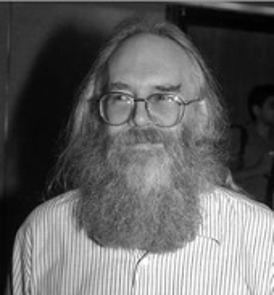
\includegraphics[width=5cm]{pictures/secret.jpg}
    \caption{L'image cachée} 
\end{figure}
\newline
En faisant une rapide recherche d'image inversée sur Google, on a découvert qu'il s'agit en fait de Jonathan Bruce Postel, dit Jon Postel, un célèbre informaticien qui a contribué à la création d'Internet. \\
%question 3
Maintenant que nous avons décodé l'image dans la question précédente, nous allons faire la procédure inverse : nous allons recréer l'image que nous venons de décoder. Dans la question précédente, nous avons pris l'image transporteur.bmp et nous en avons décoder l'image jon\_postel.jpg. Désormais, nous allons nous servir de l'image originel.bmp dans laquelle nous allons encoder l'image jon\_postel.jpg pour reconstituer le fichier transporteur.bmp. \\
Voici le code correspondant
\begin{lstlisting}[style=languageClarge, caption=Encodage d'un jpg secret dans une image bmp]
FILE *fsource = fopen(file_source, "r");
FILE *fsecret = fopen(file_secret, "r"); // file extrait de transporteur.bmp avec decode_bmp() -> transporteur.bmp_source.jpg

char *remake = malloc(strlen(file_secret) + strlen("_remake.bmp") + 1);
char *second = malloc(strlen("_remake.bmp") + 1);
strcpy(remake, file_secret);
strcpy(second, "_remake.bmp");
FILE *ftransp = fopen(strcat(remake, second), "w"); // nouveau fichier

char temp = fgetc(fsecret); 

fichierEntete *header = malloc(sizeof(fichierEntete));
imageEntete *imageHeader = malloc(sizeof(imageEntete));

fread(header, 1, sizeof(fichierEntete), fsource); // c'est l'inverse entre le 1 et le sizeof !!
fwrite(header, 1, sizeof(fichierEntete), ftransp);

fread(imageHeader, 1, sizeof(imageEntete), fsource);
fwrite(imageHeader, 1, sizeof(imageEntete), ftransp);

int new_bmp_size = 0;
char octet_source;
int bin_secret[8];

unsigned char char_secret = 0;
char new_octet_in_src = 0;

//Get file length
fseek(fsecret, 0, SEEK_END);
long fileLen = ftell(fsecret);
fseek(fsecret, 0, SEEK_SET);

for(int counter = 0; counter < fileLen; counter += 1) {
    char_secret = fgetc(fsecret);
    int_to_bin(char_secret, bin_secret);
    for(int i = 0; i < 8; i++) {
        octet_source = fgetc(fsource);
        new_octet_in_src = set_bit_faible(octet_source, bin_secret[7-i]);
        fputc(new_octet_in_src, ftransp);
    }
    for(int i = 0; i < 8; i++) {
        bin_secret[i] = 0;
    }
}

fclose(fsource);
fclose(fsecret);
fclose(ftransp);

printf("Secret file '%s' successfully encoded in '%s' with '%s' as original file\n\n", file_secret, remake, file_source);

return remake;
\end{lstlisting}

\begin{lstlisting}[style=languageClarge, caption=Fonction \texttt{set\_bit\_faible}]
char set_bit_faible(char octet, char bit) {
    char mask = 1;
    if(bit == 1) {
        return octet | mask;
    } else {
        return octet & ~mask;
    }
}
\end{lstlisting}

On a donc bien réussi à faire ce que l'on voulait et pour vérifier, on peut se reservir de la fonction de décodage pour décoder le fichier que l'on vient d'encoder et vérifier que l'on obtient bien l'image secrete !

\section{Conclusion}
Nous avons donc terminé ce TP, voici le code inséré dans la fonction main pour faire toutes les actions d'un coup :
\begin{lstlisting}[style=languageClarge, caption=Fonction main]
file_odd(100);

char *filename;
printf("Fichier voyelles : vowels.txt\n");
int counter = file_count_vowels("./vowels.txt");
printf("Le nombre de voyelle dans le fichier est : %d\n\n", counter);

readable_txt("utils/transporteur.txt");

char *secret_file = decode_bmp("utils/transporteur.bmp");
char *file_encode = encode_file("utils/originel.bmp", secret_file);

decode_bmp(file_encode);
\end{lstlisting}

Nous avons beaucoup apprécié faire ce TP qui nous as appris beaucoup de techniques de stéganographie. Il a été très enrichissant car nous n'avons pas l'habitude de manipuler les fichiers à ce point en lisant seulement certains octet afin de créer ou des nouveaux fichiers encodés ou décodés par exemple donc c'était une bonne expérience ! \\
Nous pouvons donc maintenant nous envoyer des images secrètes avec nos propres fonctions d'encodage et ça, c'est cool !
\end{document}
